
\chapter{Strumenti di sviluppo}\makeatletter\def\@currentlabel{2}\makeatother
\label{cap2}
\lhead{\textbf{CAPITOLO 2.} \textit{ STRUMENTI DI SVILUPPO}}

\section{Organizzazione dell'applicativo}\label{Organizzazione}
Una volta compreso il funzionamento e le peculiarità della tecnologia Blockchain, ci indentriamo nello sviluppo vero e proprio dell'applicazione.
Come anticipato, l'applicazione è una Dapp DeFi strutturata sulla rete Ethereum (per la precisione sulla rete di test Ropsten.); composta da un front-end in React e un back-end formato da smart-contract (memorizzati su Blockchain) scritti in Solidity, il quale, ci consente di distribuire l'applicazione sia su mainnet Ethereum che su qualsiasi altra Blockchain EVM compatibile. In questo capitolo verrà mostrato come le due controparti sono collegate tra di loro e tutte le tecnologie specifiche utilizzate.

\section{Tecnologie per il back-end}\label{back-end}
In una Dapp, gli smart-contract “sostituiscono” il back-end delle applicazioni tradizionali per evitare i server centralizzati e agire in modo distribuito (P2P),invece che utilizzare il protocollo HTTP per comunicare.
Gli smart-contract di Ethereum consentono di costruire architetture in cui una rete di contratti si trasmette dati tra loro, leggendo e scrivendo le proprie variabili di stato man mano che procedono, con la loro complessità limitata solo dal solo \textit{block gas limit}\footnote{Il limite di gas definisce il limite superiore del gas destinato al consumo di una transazione o per l'intero blocco.}.
Deve essere, inoltre, considerato che uno smart-contract è impossibile da modificare dopo essere stato distribuito, può soltanto essere cancellato se è stata aggiunta in precedenza una particolare funzione(per la precisione la SELFDESTRUCT opcode\footnote{un'operazione a livello della EVM, indipendente dal tipo di linguaggio o client che stai utilizzando}).

\subsection{Node.js}\label{nodeJS}
Node.js è un ambiente di runtime JavaScript open source usato per eseguire codice JavaScript all'esterno di un browser web. Ai fini del nostro progetto, node.js ci servirà per il Node Package Manager (NPM) come pre-requisito all'installazione di Truffle (\ref{Truffle}), del React App (\ref{React}) e della libreria web3.js (\ref{web3_Library}). 
\subsection{Solidity}\label{Solidity}
Per l'implementazione degli smart-contract su rete Ethereum si utilizza Solidity,  un linguaggio di programmazione object-oriented\footnote{Letteralmente “orientato agli oggetti”. L'object orientation è un paradigma di programmazione che si basa sul concetto di classi e oggetti.} designato specificamente per il loro sviluppo (vengono eseguiti sulla macchina virtuale di Ethereum)\cite{Solidity_docs}. Questo linguaggio (che è di alto livello) è stato pensato per rendere più semplice la scrittura di smart-contract, i quali, devono essere compilati in bytecode EVM (ossia codice di basso livello interpretabile solo dalla macchina e non dall'uomo).

Per fare questo, c'è bisogno di un Contract ABI (o Application Binary Interface), ossia un'interfaccia che permette di interagire con uno smart-contract tramite uno schema standard, definendo i nomi delle funzioni e i tipi di dati degli argomenti. L'ABI, infatti, è scritto in formato JSON\footnote{Acronimo di JavaScript Object Notation, è un formato standard utilizzato per lo scambio e la memorizzazione di dati sottoforma di coppie o array attributo-valore.}.

Nella nostra Dapp, dunque, quando si vogliono inserire o leggere dei dati sulla Blockchain, le funzioni chiamate devono passare sempre per l'ABI che fa da intermediatore con l'EVM. Si mostra in figura \ref{contratti_img} il processo illustrato graficamente.

\begin{figure}[h]
    \centering
    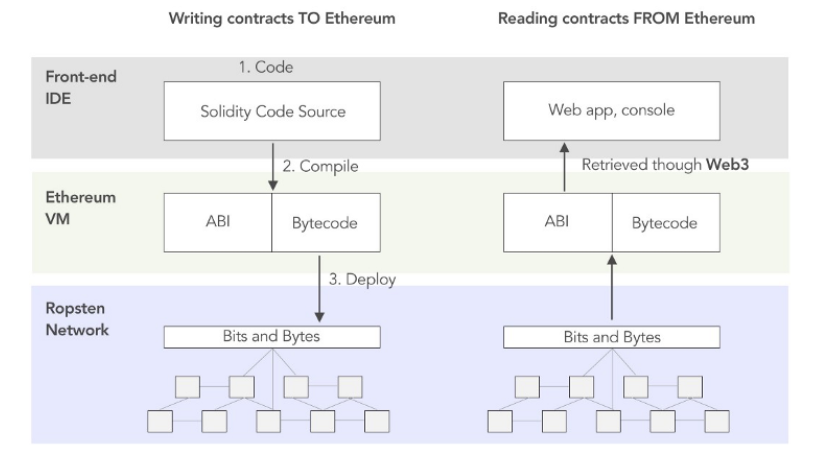
\includegraphics[width=13cm,height=8cm]{Immagini/Contratti_ETH.png}
    \caption[Rappresentazione grafica del processo di lettura/scrittura delle funzioni di uno smart-contract]{Processo di lettura/scrittura delle funzioni di uno smart-contract.}
    \label{contratti_img}
\end{figure}

Un vantaggio di Solidity è che i codici sorgente realizzati sono accessibili pubblicamente nella Blockchain di Ethereum (consultabili su qualsiasi block explorer, ossia: come detto in \cite{block_explorer}: “è uno strumento che fornisce analisi dettagliate su una rete Blockchain[...]”, esso funge da un motore di ricerca  nel quale si possono controllare i singoli blocchi, le transazioni e gli indirizzi pubblici). Per quanto riguarda la visualizzazione di questi codici: se essi sono verificati, viene mostrato il codice sorgente, altrimenti vengono mostrati in bytecode.

Solidity oltre ad essere stato uno dei primi linguaggi di programmazione smart-contract, è il più utilizzato al momento per il suo scopo e viene considerato, inoltre, il più versatile tra tutti.
\subsection{Truffle framework}\label{Truffle}
Durante l'intero ciclo di vita del progetto, è stato utilizzato il framework Truffle della Truffle Suite di Consensys\footnote{Una delle principali aziende di sviluppo software Blockchain di Ethereum.}\cite{Truffle_Suite} per il supporto allo sviluppo e alla distribuzione degli smart-contract permettendo di comunicare con essi, senza faticose programmazioni lato client. Truffle permette diverse funzioni:
\begin{figure}[h]
    \centering
    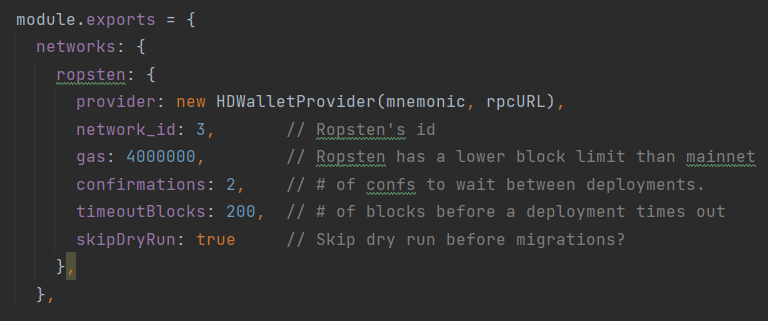
\includegraphics[width=13cm,height=6cm]{Immagini/truffle_config.png}
    \caption[File di configurazione truffle-config.js]{File di configurazione \textit{truffle-config.js} per la testnet Ropsten.}
    \label{truffle_config}
\end{figure}
\begin{itemize}
\item Gestire i propri contratti collegando librerie e diverse applicazioni Ethereum;
\item Automatizzazione del testing dei contratti per uno sviluppo più rapido;
\item Distribuzione e Migrazione degli script. La migrazione aiuta i contratti ad essere distribuiti e salvati sulla rete Ethereum, Truffle gestisce le migrazioni tramite dei file Javascript \footnote{Linguaggio di programmazione multi paradigma orientato agli eventi.}, i quali, da documentazione \cite{Truffle_migration}:“[...]sono responsabili della gestione temporanea delle attività di distribuzione e vengono scritti partendo dal presupposto che le esigenze di distribuzione cambieranno nel tempo.[...]”;
\item Fornisce una console interattiva per compilare, testare o debuggare\footnote{Procedura molto importante che permette di facilitare  la ricerca di errori logici all'interno del programma, viene effettuato attraverso un' altro programma chiamato debugger.} i propri contratti.
\end{itemize}

Truffle distribuisce l'applicazione su un nodo che rappresenta la rete (Blockchain) specifica da voler utilizzare; il tutto viene definito in un unico file Javascript di configurazione chiamato \textit{truffle-config.js}.
Nel nostro caso l'applicazione è stata distribuita sulla rete di test Ropsten di Ethereum, il file di configurazione è mostrato in figura \ref{truffle_config}.

\section{Tecnologie per il Front-end}\label{front-end}
A differenza del back-end, in una Dapp il funzionamento lato front-end e l'interfaccia utente (UI) non cambiano rispetto una web-app tradizionale, l'unica differenza la fa l'interazione con il back-end.
La gestione delle interazioni con la rete Ethereum nell'applicazione vengono assegnate alla libreria Javascript \textit{web3.js} e all'estensione del browser \textit{Metamask} (spiegati nei paragrafi successivi).

\subsection{React}\label{React}
La nostra applicazione è stata realizzata interamente in \textit{React}\cite{React}, una libreria Javascript per la creazione di UI sviluppata nel 2013 da Facebook; la libreria è ora open-source ed è sostenuta da una vasta comunità di programmatori. 
React permette di creare interfacce dinamiche complesse che allo stesso tempo risultano essere semplici e intuitive da utilizzare.

Come è ormai risaputo, per la creazione di applicazioni Web è necessario coinvolgere i tre linguaggi fondamentali:
\begin{itemize}
\item HTML ( o Hypertext Markup Language) per strutturare il sito web;
\item CSS (o Cascading Style Sheets) per la resa grafica dell'applicazione;
\item Javascript, invece, per la logica applicativa e per rendere interattive le applicazioni web.
\end{itemize}

Nelle applicazioni \textit{React}, tutto questo viene semplificato nella sintassi JSX (Javascript XML), un'estensione della sintassi di Javascript, che ci permette di inserire delle strutture simili ad HTML nello stesso file in cui si scrive la logica Javascript. L'uso di JSX, seppur non obbligatorio, permette una più facile lettura degli elementi e dei suoi attributi. Questo particolare tipo di sintassi non è decifrabile nativamente dai browser web e c'è bisogno di un pre-compilatore per rendere leggibile il tutto; la libreria \textit{React}, oggi come oggi, utilizza Babel\footnote{Compiler Javascript.} per questo scopo.

Una delle peculiarità di React è quella di comporre le sue applicazioni di \textit{componenti} riutilizzabili permettendo di semplificare lo sviluppo, di non ripetere frazioni di codice più volte e di importare un determinato componente solo quando è davvero necessario.
Ogni componente può essere personalizzato a proprio piacimento incorporando un CSS specifico.

\subsection{La libreria Web3.js}\label{web3_Library}
Come anticipato nei paragrafi precedenti, la libreria \textit{web3.js}\cite{web3API} viene utilizzata per l'interazione con gli smart-contract su Ethereum.

Come viene espresso in \cite{web3API} web3.js è :“una raccolta di librerie che consentono di interagire con un nodo Ethereum locale o remoto utilizzando HTTP, IPC o WebSocket.”, essa è l'API\footnote{Abbreviazione di Application Programming Interface, è un'interfaccia composta di definizioni e protocolli per la creazione e l'integrazione di software applicativi.} Javascript ufficiale di Ethereum.
Prima di definire nel dettaglio il funzionamento e le caratteristiche di questa libreria, introduciamo brevemente il concetto di JSON-RPC.

JSON-RPC (Remote Procedure Call Protocol) è un protocollo per la chiamata di procedure remote,  nelle quali è possibile passare anche oggetti complessi e ricevere come output dati multipli. I codici di successo e di errore sono standardizzati, in maniera tale da renderne più facile la comprensione.

Questo servizio viene interrogato tramite HTTP o TCP/IP e restituisce una serializzazione del risultato in formato JSON. Ogni richiesta è caratterizzata dalle seguenti componenti:
\begin{itemize}
\item method: Stringa contenente il nome del metodo che la richiesta deve invocare;
\item params: Corrisponde ai parametri da passare al metodo sotto forma di array di oggetti;
\item id: un valore univoco utilizzato per abbinare la risposta alla richiesta.
\end{itemize}

Presso questa fonte sono consultabili tutti i metodi del JSON-RPC di Ethereum : \cite{eth_rpc}.
La libreria web3.js comunica con la Blockchain di Ethereum proprio grazie al JSON-RPC, infatti, quest'ultima legge e scrive i dati effettuando richieste JSON-RPC a un nodo Ethereum.
Nel progetto di questo elaborato verranno utilizzati principalmente due pacchetti specifici di web3.js:
\begin{itemize}
\item web3.eth: pacchetto utilizzato per interagire a tutti gli effetti con la rete Ethereum e gli smart-contract;
\item web3.utils: pacchetto contenente diverse funzioni per la conversione di stringhe e numeri in formati specifici.
\end{itemize}

\subsection{Metamask}\label{metamask}
Per sfruttare al meglio la libreria web3.js e semplificarne l'utilizzo c'è bisogno di utilizzare un provider\footnote{Anche chiamato Internet service provider (ISP) indica un'organizzazione o un'infrastruttura che offre servizi (inerenti a Internet) agli utenti.}.Senza di esso un semplice utente avrebbe molta più difficoltà a comunicare con la Blockchain.
Il provider scelto per l'elaborato è \textit{Metamask}. 

\textit{Metamask} è un \textit{wallet}(ossia un portafoglio digitale) utilizzato per la custodia dei propri asset (nel nostro caso criptovalute) e per comunicare con applicazioni decentralizzate. Esso può essere utilizzato direttamente dal proprio browser tramite un'estensione, semplificando al massimo la fruizione dei servizi offerti da una Dapp. Una volta installata questa estensione, Metamask istanzierà un oggetto Ethereum alla finestra principale del browser, la quale presenza è verificabile tramite web3.js. 
A questo punto l'utente potrà eseguire tutte le operazioni che la Dapp gli consente di fare e Metamask gestirà tutte le transazioni associate.

